\documentclass[]{tufte-handout}

% ams
\usepackage{amssymb,amsmath}

\usepackage{ifxetex,ifluatex}
\usepackage{fixltx2e} % provides \textsubscript
\ifnum 0\ifxetex 1\fi\ifluatex 1\fi=0 % if pdftex
  \usepackage[T1]{fontenc}
  \usepackage[utf8]{inputenc}
\else % if luatex or xelatex
  \makeatletter
  \@ifpackageloaded{fontspec}{}{\usepackage{fontspec}}
  \makeatother
  \defaultfontfeatures{Ligatures=TeX,Scale=MatchLowercase}
  \makeatletter
  \@ifpackageloaded{soul}{
     \renewcommand\allcapsspacing[1]{{\addfontfeature{LetterSpace=15}#1}}
     \renewcommand\smallcapsspacing[1]{{\addfontfeature{LetterSpace=10}#1}}
   }{}
  \makeatother

\fi

% graphix
\usepackage{graphicx}
\setkeys{Gin}{width=\linewidth,totalheight=\textheight,keepaspectratio}

% booktabs
\usepackage{booktabs}

% url
\usepackage{url}

% hyperref
\usepackage{hyperref}

% units.
\usepackage{units}


\setcounter{secnumdepth}{-1}

% citations

% pandoc syntax highlighting
\usepackage{color}
\usepackage{fancyvrb}
\newcommand{\VerbBar}{|}
\newcommand{\VERB}{\Verb[commandchars=\\\{\}]}
\DefineVerbatimEnvironment{Highlighting}{Verbatim}{commandchars=\\\{\}}
% Add ',fontsize=\small' for more characters per line
\newenvironment{Shaded}{}{}
\newcommand{\AlertTok}[1]{\textcolor[rgb]{1.00,0.00,0.00}{\textbf{#1}}}
\newcommand{\AnnotationTok}[1]{\textcolor[rgb]{0.38,0.63,0.69}{\textbf{\textit{#1}}}}
\newcommand{\AttributeTok}[1]{\textcolor[rgb]{0.49,0.56,0.16}{#1}}
\newcommand{\BaseNTok}[1]{\textcolor[rgb]{0.25,0.63,0.44}{#1}}
\newcommand{\BuiltInTok}[1]{#1}
\newcommand{\CharTok}[1]{\textcolor[rgb]{0.25,0.44,0.63}{#1}}
\newcommand{\CommentTok}[1]{\textcolor[rgb]{0.38,0.63,0.69}{\textit{#1}}}
\newcommand{\CommentVarTok}[1]{\textcolor[rgb]{0.38,0.63,0.69}{\textbf{\textit{#1}}}}
\newcommand{\ConstantTok}[1]{\textcolor[rgb]{0.53,0.00,0.00}{#1}}
\newcommand{\ControlFlowTok}[1]{\textcolor[rgb]{0.00,0.44,0.13}{\textbf{#1}}}
\newcommand{\DataTypeTok}[1]{\textcolor[rgb]{0.56,0.13,0.00}{#1}}
\newcommand{\DecValTok}[1]{\textcolor[rgb]{0.25,0.63,0.44}{#1}}
\newcommand{\DocumentationTok}[1]{\textcolor[rgb]{0.73,0.13,0.13}{\textit{#1}}}
\newcommand{\ErrorTok}[1]{\textcolor[rgb]{1.00,0.00,0.00}{\textbf{#1}}}
\newcommand{\ExtensionTok}[1]{#1}
\newcommand{\FloatTok}[1]{\textcolor[rgb]{0.25,0.63,0.44}{#1}}
\newcommand{\FunctionTok}[1]{\textcolor[rgb]{0.02,0.16,0.49}{#1}}
\newcommand{\ImportTok}[1]{#1}
\newcommand{\InformationTok}[1]{\textcolor[rgb]{0.38,0.63,0.69}{\textbf{\textit{#1}}}}
\newcommand{\KeywordTok}[1]{\textcolor[rgb]{0.00,0.44,0.13}{\textbf{#1}}}
\newcommand{\NormalTok}[1]{#1}
\newcommand{\OperatorTok}[1]{\textcolor[rgb]{0.40,0.40,0.40}{#1}}
\newcommand{\OtherTok}[1]{\textcolor[rgb]{0.00,0.44,0.13}{#1}}
\newcommand{\PreprocessorTok}[1]{\textcolor[rgb]{0.74,0.48,0.00}{#1}}
\newcommand{\RegionMarkerTok}[1]{#1}
\newcommand{\SpecialCharTok}[1]{\textcolor[rgb]{0.25,0.44,0.63}{#1}}
\newcommand{\SpecialStringTok}[1]{\textcolor[rgb]{0.73,0.40,0.53}{#1}}
\newcommand{\StringTok}[1]{\textcolor[rgb]{0.25,0.44,0.63}{#1}}
\newcommand{\VariableTok}[1]{\textcolor[rgb]{0.10,0.09,0.49}{#1}}
\newcommand{\VerbatimStringTok}[1]{\textcolor[rgb]{0.25,0.44,0.63}{#1}}
\newcommand{\WarningTok}[1]{\textcolor[rgb]{0.38,0.63,0.69}{\textbf{\textit{#1}}}}

% longtable

% multiplecol
\usepackage{multicol}

% strikeout
\usepackage[normalem]{ulem}

% morefloats
\usepackage{morefloats}


% tightlist macro required by pandoc >= 1.14
\providecommand{\tightlist}{%
  \setlength{\itemsep}{0pt}\setlength{\parskip}{0pt}}

% title / author / date
\title{Logistic regression - introduction}
\author{Ian Handel}
\date{2019-06-13}


\begin{document}

\maketitle




\hypertarget{introduction}{%
\section{Introduction}\label{introduction}}

These notes are a basic introduction to binary logistic regression used
to analyse data with binary outcomes. In these notes we'll aim to cover
the following learning outcomes:

\begin{itemize}
\tightlist
\item
  \textbf{Refresher} on logs, odds, probability and linear regression
\item
  Understand why linear regression not sensible for \textbf{binary data}
\item
  Explain how \textbf{logit} and binomial model let us \textbf{extend
  linear regression}
\item
  Be able to run a \textbf{simple logistic regression in R}
\item
  Be able to explain basic R glm \textbf{output}
\item
  Be able to explain \textbf{estimates} with categorical and continuous
  variables
\item
  Explain \textbf{significance test results} on variables
\item
  Introduce some basic ideas for \textbf{selecting variables and models}
\item
  \textbf{Things to watch out for!}
\item
  \textbf{Know where to go next!}
\end{itemize}

\hypertarget{prerequisites}{%
\section{Prerequisites}\label{prerequisites}}

We'll cover a couple of background topics but to follow these notes
you'll need to be able to load packages in R, run simple code in R and
have a basic understanding of linear regression and statistical
hypothesis tests.

\hypertarget{running-the-example-code}{%
\section{Running the example code}\label{running-the-example-code}}

To run the R code in these notes you'll need to start an rstudio
project, load in the example data-set and have a few packages downloaded
and loaded into your R session.

To download the packages (if you don't have them already) use\ldots{}

\begin{Shaded}
\begin{Highlighting}[]
\KeywordTok{install.packages}\NormalTok{(}\StringTok{"tidyverse"}\NormalTok{)}
\KeywordTok{install.packages}\NormalTok{(}\StringTok{"boot"}\NormalTok{)}
\KeywordTok{install.packages}\NormalTok{(}\StringTok{"broom"}\NormalTok{)}
\KeywordTok{install.packages}\NormalTok{(}\StringTok{"skimr"}\NormalTok{)}
\KeywordTok{install.packages}\NormalTok{(}\StringTok{"sjPlot"}\NormalTok{)}
\KeywordTok{install.packages}\NormalTok{(}\StringTok{"kableExtra"}\NormalTok{)}
\end{Highlighting}
\end{Shaded}

Start a new project in rstudio and in an rscript use the floowing code
to load the libraries you need and to import/load the data\ldots{}

Loading the packages\ldots{}

\begin{Shaded}
\begin{Highlighting}[]
\KeywordTok{library}\NormalTok{(tidyverse)}
\KeywordTok{library}\NormalTok{(boot)}
\KeywordTok{library}\NormalTok{(broom)}
\KeywordTok{library}\NormalTok{(skimr)}
\KeywordTok{library}\NormalTok{(sjPlot)}
\KeywordTok{library}\NormalTok{(kableExtra)}
\end{Highlighting}
\end{Shaded}

Loading the data (from the csv file on Basecamp)\ldots{}

\begin{Shaded}
\begin{Highlighting}[]
\NormalTok{dat <-}\StringTok{ }\KeywordTok{read_csv}\NormalTok{(}\StringTok{"logreg_data_01_20190530.csv"}\NormalTok{)}
\end{Highlighting}
\end{Shaded}

This dataset describes 500 animals giving their weight in kg, age in
days, supplement levels (mg), sex, region where they liver (A, B, C or
D) and whether they were treated with anthelmintics or not. It's a
dataset made up for this course by the way!

\hypertarget{revision-background-topics}{%
\section{Revision / background
topics}\label{revision-background-topics}}

\hypertarget{logarithms-logs}{%
\subsection{Logarithms (`logs')}\label{logarithms-logs}}

Skip this if you are happy with logs (including base `e')

`Logs' are a mathematical function that changes a number. They take the
form \(log_b(x)=y\). What this means is \(b\) to the power \(y\) will
give us \(x\). It's easier to understand with examples. Let's start with
base 10\ldots{}.

\[log_{10}(10)=1\]

\[log_{10}(1000)=3\]

\[log_{10}(0.01)=-2\]

So the logs of all the numbers in brackets are the number you'd need to
raise 10 to to get them.

We can have other bases e.g. \(e\)., \(e\) is a special mathematical
constant that feautres a lot behind the scene in statistics it's roughly
2.718\ldots{}

\[log_e(2.718)\simeq1\]

`Inverse logs' let us turn logs back into the original number. We simply
raise the `base' of our logs to the number we what to invert and we end
up with the original number. So \(log_{10}(1000)=3\) and
\(10^3=1000\)\ldots{}

One feature of logs is that adding the logs of two numbers is equivalent
to multiplying the numbers\ldots{}

\[100 \times 1000 = 100000\]

\[log_{10}(100) + log_{10}(1000) = log_{10}(100000)\]

Because \(log_{10}(100) = 2\), \(log_{10}(1000)=3\) and
\(log_{10}(100000)=5\)

If this all seems a bit too much don't worry. Just remember that adding
logs is like multiplying numbers and you'll be fine!

\hypertarget{odds-and-probability}{%
\section{Odds and probability}\label{odds-and-probability}}

\textbf{Probabilities} have values from 0 (`never happens') to 1
(`always happens')

\textbf{`events of interest' ÷ `all events'}

What is the probability that a fair coin lands on heads?

\[1/2 = 0.5\]

What is the probability that a 6 sided die lands on 4?

\[1/6 \simeq 0.166\]

\textbf{Odds} have values from 0 (`never happen') to infinity (`always
happens')

\textbf{`events of interest' ÷ `other events'}

What are the odds that a fair coin lands on heads?

\[1/1 = 1\]

What are the odds that a 6 sided die lands on 4?

\[1/5 = 0.2\]

\newpage

\hypertarget{linear-regression}{%
\section{Linear regression}\label{linear-regression}}

Remember that linear regression is a statistical method that lets us
understand and predict numerical outcomes using one or more predictor
variables. The predictor variables may be numerical or categorical.
Linear regression also assumes there's a linear i.e.~straight line
relationship between the predictor numerical variable sand the outcome.
Using the data set we have loaded we can plot weight against age and sex
and see that there looks to be a linear relationship between age and
weight for each sex\ldots{}

\begin{Shaded}
\begin{Highlighting}[]
\NormalTok{fig1 <-}\StringTok{ }\KeywordTok{ggplot}\NormalTok{(dat) }\OperatorTok{+}\StringTok{ }\KeywordTok{aes}\NormalTok{(age, weight, }\DataTypeTok{colour =}\NormalTok{ sex) }\OperatorTok{+}\StringTok{ }
\StringTok{    }\KeywordTok{geom_point}\NormalTok{(}\DataTypeTok{shape =} \DecValTok{1}\NormalTok{) }\OperatorTok{+}\StringTok{ }\KeywordTok{geom_smooth}\NormalTok{(}\DataTypeTok{method =} \StringTok{"lm"}\NormalTok{, }
    \DataTypeTok{se =} \OtherTok{FALSE}\NormalTok{) }\OperatorTok{+}\StringTok{ }\KeywordTok{theme_bw}\NormalTok{() }\OperatorTok{+}\StringTok{ }\KeywordTok{labs}\NormalTok{(}\DataTypeTok{title =} \StringTok{"Weight vs Age of the animals"}\NormalTok{, }
    \DataTypeTok{subtitle =} \StringTok{"They get bigger as they age}\CharTok{\textbackslash{}n}\StringTok{and males are heavier"}\NormalTok{, }
    \DataTypeTok{x =} \StringTok{"Age (days)"}\NormalTok{, }\DataTypeTok{y =} \StringTok{"Weight (Kg)"}\NormalTok{, }\DataTypeTok{colour =} \StringTok{"Sex"}\NormalTok{)}

\KeywordTok{print}\NormalTok{(fig1)}
\end{Highlighting}
\end{Shaded}

\includegraphics{logistic_regression_notes_20190609_files/figure-latex/unnamed-chunk-7-1}

In R we can use the \texttt{lm()} function to fit a linear model to this
data. Normally we store the results of using the function in an R object
and look at it using `\texttt{summary()}. We can also get a tidier
output using \texttt{get\_model\_data()} from the \texttt{sjPlot}
package. Here we make a linear model predicting the animal's weight from
their age (a numerical variable) and their sex (a categorical variable).

\begin{Shaded}
\begin{Highlighting}[]
\NormalTok{mod1 <-}\StringTok{ }\KeywordTok{lm}\NormalTok{(weight }\OperatorTok{~}\StringTok{ }\NormalTok{age }\OperatorTok{+}\StringTok{ }\NormalTok{sex, }\DataTypeTok{data =}\NormalTok{ dat)}
\end{Highlighting}
\end{Shaded}

Using \texttt{summary()} from base-R\ldots{}

\begin{Shaded}
\begin{Highlighting}[]
\KeywordTok{summary}\NormalTok{(mod1)}
\end{Highlighting}
\end{Shaded}

\begin{verbatim}

Call:
lm(formula = weight ~ age + sex, data = dat)

Residuals:
    Min      1Q  Median      3Q     Max 
-2.3506 -0.4732 -0.0509  0.4572  2.0223 

Coefficients:
            Estimate Std. Error t value
(Intercept) 49.93305    0.40486  123.33
age          0.12045    0.00191   63.07
sexmale      3.51683    0.06541   53.76
            Pr(>|t|)    
(Intercept)   <2e-16 ***
age           <2e-16 ***
sexmale       <2e-16 ***
---
Signif. codes:  
  0 '***' 0.001 '**' 0.01 '*' 0.05 '.' 0.1  ' ' 1

Residual standard error: 0.7312 on 497 degrees of freedom
Multiple R-squared:  0.932, Adjusted R-squared:  0.9317 
F-statistic:  3404 on 2 and 497 DF,  p-value: < 2.2e-16
\end{verbatim}

Using \texttt{get\_model\_data()} from \texttt{sjPlot} package and
selecting the output columns we want\ldots{}

\begin{Shaded}
\begin{Highlighting}[]
\KeywordTok{get_model_data}\NormalTok{(mod1) }\OperatorTok\StringTok{ }\KeywordTok{select}\NormalTok{(term}\OperatorTok{:}\NormalTok{p.stars) }\OperatorTok\StringTok{ }
\StringTok{    }\KeywordTok{print}\NormalTok{()}
\end{Highlighting}
\end{Shaded}

\begin{verbatim}
# A tibble: 2 x 8
  term  estimate std.error statistic
  <fct>    <dbl>     <dbl>     <dbl>
1 age      0.120   0.00191      63.1
2 sexm~    3.52    0.0654       53.8
# ... with 4 more variables: p.value <dbl>,
#   conf.low <dbl>, conf.high <dbl>,
#   p.stars <chr>
\end{verbatim}

The analysis suggestes that both \textbf{age} and \textbf{sex} are
significant predcitors of weight. Weight increasing by about 0.12 Kg per
day of age and that males are about 3.5 Kg heavier than females.

\newpage

\hypertarget{analysing-binary-data}{%
\section{Analysing binary data}\label{analysing-binary-data}}

Binary data common in epidemiology e.g.~disease status (diseased or
healthy), life (alive or dead) etc. In the example dataset we have the
column \texttt{status} where animals can be either \textbf{healthy} or
\textbf{diseased}.

\begin{tabular}{l|l|r|l|r|l|r|l}
\hline
ID & treatment & age & region & supp & sex & weight & status\\
\hline
A0049 & control & 221 & D & 7.891 & male & 80.9 & diseased\\
\hline
A0485 & control & 220 & A & 2.651 & male & 79.5 & diseased\\
\hline
A0321 & treated & 238 & B & 1.671 & male & 82.2 & diseased\\
\hline
A0153 & treated & 183 & C & 6.346 & female & 71.7 & healthy\\
\hline
A0074 & treated & 187 & A & 9.655 & male & 77.0 & diseased\\
\hline
A0228 & control & 206 & C & 8.046 & female & 74.7 & diseased\\
\hline
\end{tabular}

As we know that some animals were treated with an anthelmintic and some
were not it may be interesting to look at the number of healhty and
diseased animals in the treated and control (untreated) groups\ldots{}

\begin{tabular}{l|r|r}
\hline
treatment & diseased & healthy\\
\hline
control & 154 & 44\\
\hline
treated & 209 & 93\\
\hline
\end{tabular}

\begin{Shaded}
\begin{Highlighting}[]
\KeywordTok{with}\NormalTok{(dat, \{}
\NormalTok{    \{}
        \KeywordTok{fisher.test}\NormalTok{(status, treatment)}
\NormalTok{    \}}
\NormalTok{\})}
\end{Highlighting}
\end{Shaded}

\begin{verbatim}

    Fisher's Exact Test for Count Data

data:  status and treatment
p-value = 0.04032
alternative hypothesis: true odds ratio is not equal to 1
95 percent confidence interval:
 1.010694 2.419528
sample estimates:
odds ratio 
  1.556051 
\end{verbatim}

\hypertarget{multivariable-analysis}{%
\section{Multivariable analysis}\label{multivariable-analysis}}

How about recoding the outcome as 0/1?

\begin{tabular}{l|l|r|l|r|l|r|l|r}
\hline
ID & treatment & age & region & supp & sex & weight & status & status01\\
\hline
A0049 & control & 221 & D & 7.891 & male & 80.9 & diseased & 1\\
\hline
A0485 & control & 220 & A & 2.651 & male & 79.5 & diseased & 1\\
\hline
A0321 & treated & 238 & B & 1.671 & male & 82.2 & diseased & 1\\
\hline
A0153 & treated & 183 & C & 6.346 & female & 71.7 & healthy & 0\\
\hline
A0074 & treated & 187 & A & 9.655 & male & 77.0 & diseased & 1\\
\hline
A0228 & control & 206 & C & 8.046 & female & 74.7 & diseased & 1\\
\hline
\end{tabular}

Then use linear regression\ldots{}

\hypertarget{linear-regression-1}{%
\section{Linear regression 1}\label{linear-regression-1}}

\includegraphics{logistic_regression_notes_20190609_files/figure-latex/unnamed-chunk-15-1}

\hypertarget{linear-regression-2}{%
\section{Linear regression 2}\label{linear-regression-2}}

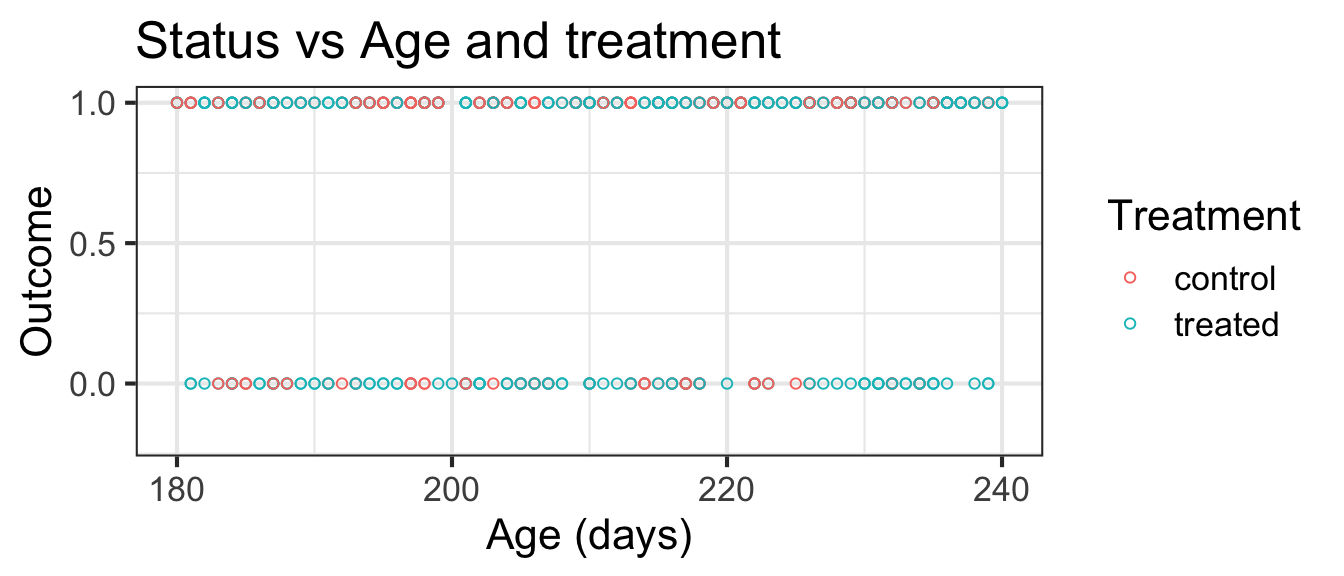
\includegraphics{logistic_regression_notes_20190609_files/figure-latex/unnamed-chunk-16-1}

\hypertarget{problems}{%
\subsection{Problems}\label{problems}}

-predicts (impossible) intermediate values

-can predict \textless{}0 and \textgreater{}1

\hypertarget{so-how-do-we-fix-this}{%
\section{So how do we fix this?}\label{so-how-do-we-fix-this}}

\textbf{Linear regression does this\ldots{}}

\(weight \sim \beta_0 + \beta_1 age + \beta_2 sex + \epsilon\)

or in english\ldots{}

The outcome, \(weight\), is related to the predictors

by one or more straight lines.

\begin{Shaded}
\begin{Highlighting}[]
\KeywordTok{print}\NormalTok{(fig1)}
\end{Highlighting}
\end{Shaded}

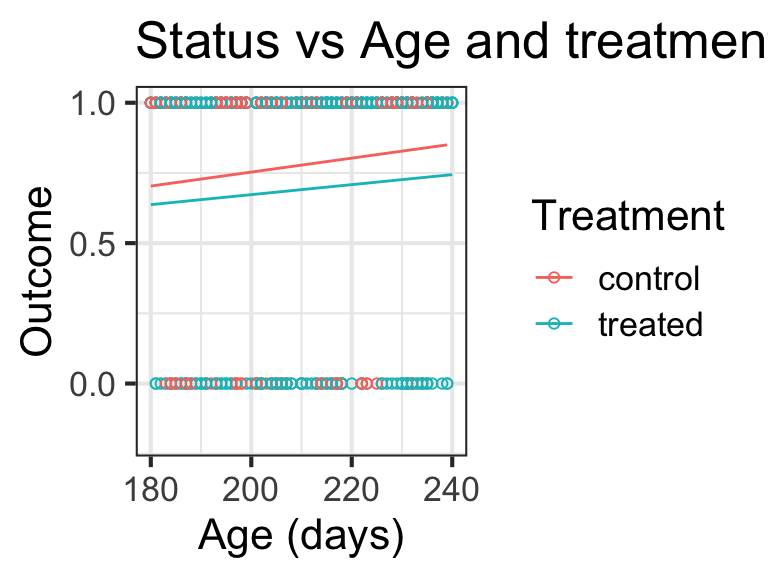
\includegraphics{logistic_regression_notes_20190609_files/figure-latex/unnamed-chunk-17-1}

\textbf{For binary data we want}

Our outcome to be 0 or 1

So rather than modelling the outcome.

We model the \textbf{probability} of something e.g.~being
diseased\ldots{}

\hypertarget{the-logistic-bit}{%
\section{The logistic bit\ldots{}}\label{the-logistic-bit}}

Linear regression models model numbers, any numbers!

Probabilities go from\ldots{}

0 to 1

So we need to turn any number into 0 - 1

\begin{center}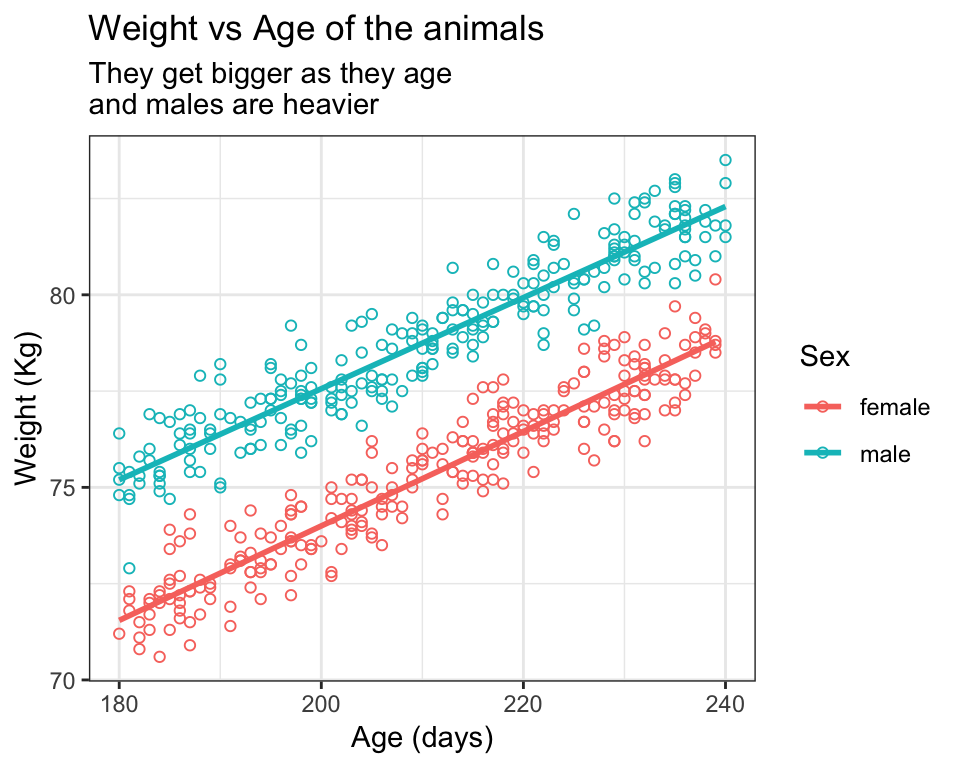
\includegraphics{logistic_regression_notes_20190609_files/figure-latex/unnamed-chunk-18-1} \end{center}

In fact the regression value is the log of the odds of the outcome.

\#The logistic bit 2

So we have an outcome, e.g.~being diseased vs healthy, that is coded 0
or 1

And our model is

\[ log_e(\frac{prob}{1 - prob}) \sim \beta_0 + \beta_1 age + \beta_2 treatment) \]

or in english

\textbf{The log of the odds of an animal being diseased are modelled by
a linear combination of the predictor variables}

\hypertarget{worked-example-in-r}{%
\section{Worked example in R}\label{worked-example-in-r}}

\hypertarget{r-code-for-logistic-regression}{%
\section{R code for logistic
regression}\label{r-code-for-logistic-regression}}

\begin{Shaded}
\begin{Highlighting}[]
\KeywordTok{head}\NormalTok{(dat)}
\end{Highlighting}
\end{Shaded}

\begin{table}[H]
\centering\begingroup\fontsize{8}{10}\selectfont

\begin{tabular}{l|l|r|l|r|l|r|l|r}
\hline
ID & treatment & age & region & supp & sex & weight & status & status01\\
\hline
A0001 & treated & 219 & D & 6.731 & female & 76.2 & diseased & 1\\
\hline
A0002 & treated & 218 & C & 7.950 & female & 76.0 & diseased & 1\\
\hline
A0003 & control & 214 & A & 5.617 & female & 75.3 & healthy & 0\\
\hline
A0004 & control & 194 & A & 8.490 & female & 72.1 & diseased & 1\\
\hline
A0005 & treated & 185 & D & 7.127 & female & 72.6 & healthy & 0\\
\hline
A0006 & treated & 235 & A & 4.882 & female & 77.8 & healthy & 0\\
\hline
\end{tabular}
\endgroup{}
\end{table}

A linear model of weight

\begin{Shaded}
\begin{Highlighting}[]
\NormalTok{mod_weight <-}\StringTok{ }\KeywordTok{lm}\NormalTok{(weight }\OperatorTok{~}\StringTok{ }\NormalTok{age }\OperatorTok{+}\StringTok{ }\NormalTok{sex, }\DataTypeTok{data =}\NormalTok{ dat)}
\end{Highlighting}
\end{Shaded}

A logistic regression model of disease status

\begin{Shaded}
\begin{Highlighting}[]
\NormalTok{mod_disease <-}\StringTok{ }\KeywordTok{glm}\NormalTok{(status01 }\OperatorTok{~}\StringTok{ }\NormalTok{treatment }\OperatorTok{+}\StringTok{ }\NormalTok{age, }
    \DataTypeTok{family =}\NormalTok{ binomial, }\DataTypeTok{data =}\NormalTok{ dat)}
\end{Highlighting}
\end{Shaded}

\hypertarget{the-output}{%
\section{The output}\label{the-output}}

\begin{Shaded}
\begin{Highlighting}[]
\KeywordTok{print}\NormalTok{(}\KeywordTok{summary}\NormalTok{(mod_disease), }\DataTypeTok{digits =} \DecValTok{3}\NormalTok{)}
\end{Highlighting}
\end{Shaded}

\begin{verbatim}

Call:
glm(formula = status01 ~ treatment + age, family = binomial, 
    data = dat)

Deviance Residuals: 
   Min      1Q  Median      3Q     Max  
-1.847  -1.428   0.746   0.826   0.973  

Coefficients:
                 Estimate Std. Error z value
(Intercept)      -0.88412    1.23913   -0.71
treatmenttreated -0.45345    0.21225   -2.14
age               0.01021    0.00589    1.74
                 Pr(>|z|)  
(Intercept)         0.476  
treatmenttreated    0.033 *
age                 0.083 .
---
Signif. codes:  
  0 '***' 0.001 '**' 0.01 '*' 0.05 '.' 0.1  ' ' 1

(Dispersion parameter for binomial family taken to be 1)

    Null deviance: 587.20  on 499  degrees of freedom
Residual deviance: 579.67  on 497  degrees of freedom
AIC: 585.7

Number of Fisher Scoring iterations: 4
\end{verbatim}

\hypertarget{the-output-1}{%
\section{The output}\label{the-output-1}}

\begin{Shaded}
\begin{Highlighting}[]
\KeywordTok{print}\NormalTok{(}\KeywordTok{summary}\NormalTok{(mod_disease), }\DataTypeTok{digits =} \DecValTok{3}\NormalTok{)}
\end{Highlighting}
\end{Shaded}

\begin{verbatim}

Call:
glm(formula = status01 ~ treatment + age, family = binomial, 
    data = dat)

Deviance Residuals: 
   Min      1Q  Median      3Q     Max  
-1.847  -1.428   0.746   0.826   0.973  

Coefficients:
                 Estimate Std. Error z value
(Intercept)      -0.88412    1.23913   -0.71
treatmenttreated -0.45345    0.21225   -2.14
age               0.01021    0.00589    1.74
                 Pr(>|z|)  
(Intercept)         0.476  
treatmenttreated    0.033 *
age                 0.083 .
---
Signif. codes:  
  0 '***' 0.001 '**' 0.01 '*' 0.05 '.' 0.1  ' ' 1

(Dispersion parameter for binomial family taken to be 1)

    Null deviance: 587.20  on 499  degrees of freedom
Residual deviance: 579.67  on 497  degrees of freedom
AIC: 585.7

Number of Fisher Scoring iterations: 4
\end{verbatim}

\hypertarget{the-output-2}{%
\section{The output}\label{the-output-2}}

Lets get 'tidy output\ldots{}

\begin{Shaded}
\begin{Highlighting}[]
\KeywordTok{tidy}\NormalTok{(mod_disease)  }\CommentTok{#tidy from the broom package}
\end{Highlighting}
\end{Shaded}

\begin{verbatim}
# A tibble: 3 x 5
  term   estimate std.error statistic p.value
  <chr>     <dbl>     <dbl>     <dbl>   <dbl>
1 (Inte~  -0.884    1.24       -0.714  0.476 
2 treat~  -0.453    0.212      -2.14   0.0326
3 age      0.0102   0.00589     1.74   0.0827
\end{verbatim}

\hypertarget{odds-ratios}{%
\section{odds ratios}\label{odds-ratios}}

The estimates = log(odds ratios)

i.e.

\[\frac{odds\ of\ outcome\ if\ have\ factor}{odds\ of\ outcome\ if\ dont\ have\ factor}\]

So we get odds ratios by `inverse logging them'.

We can remove the intercept.

\begin{Shaded}
\begin{Highlighting}[]
\KeywordTok{tidy}\NormalTok{(mod_disease) }\OperatorTok\StringTok{ }\KeywordTok{filter}\NormalTok{(term }\OperatorTok{!=}\StringTok{ "(Intercept)"}\NormalTok{) }\OperatorTok\StringTok{ }
\StringTok{    }\KeywordTok{mutate}\NormalTok{(}\DataTypeTok{OR =} \KeywordTok{exp}\NormalTok{(estimate))}
\end{Highlighting}
\end{Shaded}

\begin{verbatim}
# A tibble: 2 x 6
  term  estimate std.error statistic p.value
  <chr>    <dbl>     <dbl>     <dbl>   <dbl>
1 trea~  -0.453    0.212       -2.14  0.0326
2 age     0.0102   0.00589      1.74  0.0827
# ... with 1 more variable: OR <dbl>
\end{verbatim}

\hypertarget{a-results-table}{%
\section{A results table}\label{a-results-table}}

\begin{Shaded}
\begin{Highlighting}[]
\KeywordTok{tidy}\NormalTok{(mod_disease) }\OperatorTok\StringTok{ }\KeywordTok{mutate}\NormalTok{(}\DataTypeTok{OR =} \KeywordTok{exp}\NormalTok{(estimate)) }\OperatorTok\StringTok{ }
\StringTok{    }\KeywordTok{bind_cols}\NormalTok{(}\KeywordTok{exp}\NormalTok{(}\KeywordTok{confint_tidy}\NormalTok{(mod_disease)) }\OperatorTok\StringTok{ }
\StringTok{        }\KeywordTok{as_tibble}\NormalTok{()) }\OperatorTok\StringTok{ }\KeywordTok{filter}\NormalTok{(term }\OperatorTok{!=}\StringTok{ "(Intercept)"}\NormalTok{) }\OperatorTok\StringTok{ }
\StringTok{    }\KeywordTok{select}\NormalTok{(term, OR, conf.low, conf.high, p.value)}
\end{Highlighting}
\end{Shaded}

\begin{tabular}{l|r|r|r|r}
\hline
term & OR & conf.low & conf.high & p.value\\
\hline
treatmenttreated & 0.635434 & 0.4165578 & 0.9586278 & 0.0326443\\
\hline
age & 1.010266 & 0.9987142 & 1.0220622 & 0.0827082\\
\hline
\end{tabular}

But what does it mean?

\hypertarget{interpreting-the-odds-ratios}{%
\section{Interpreting the odds
ratios}\label{interpreting-the-odds-ratios}}

\begin{tabular}{l|r|r|r|r}
\hline
term & OR & 2.5 \% & 97.5 \% & p.value\\
\hline
treatmenttreated & 0.635434 & 0.4165578 & 0.9586278 & 0.0326443\\
\hline
age & 1.010266 & 0.9987142 & 1.0220622 & 0.0827082\\
\hline
\end{tabular}

\hypertarget{odds-ratios-multiply}{%
\subsection{\texorpdfstring{Odds ratios
\textbf{multiply}}{Odds ratios multiply}}\label{odds-ratios-multiply}}

\hypertarget{categorical-predictors}{%
\subsection{Categorical predictors}\label{categorical-predictors}}

How many times greater the odds of outcome are \textbf{if} the risk
factor (etc) is present.

So for the treatment variable (which can be control or treatment) the
odds of disease if treated are 0.635 \textbf{times greater} than if
untreated (control).

\hypertarget{interpreting-the-odds-ratios-1}{%
\section{Interpreting the odds
ratios}\label{interpreting-the-odds-ratios-1}}

\begin{tabular}{l|r|r|r|r}
\hline
term & OR & 2.5 \% & 97.5 \% & p.value\\
\hline
treatmenttreated & 0.635434 & 0.4165578 & 0.9586278 & 0.0326443\\
\hline
age & 1.010266 & 0.9987142 & 1.0220622 & 0.0827082\\
\hline
\end{tabular}

\hypertarget{odds-ratios-multiply-1}{%
\subsection{\texorpdfstring{Odds ratios
\textbf{multiply}}{Odds ratios multiply}}\label{odds-ratios-multiply-1}}

\hypertarget{numerical-predictors}{%
\subsection{Numerical predictors}\label{numerical-predictors}}

How many times greater the odds of outcome are for \textbf{each unit
change} in the variable

So for the age variable the odds of disease are 1.01 \textbf{times
greater} for each day older.

So for 3 days it's 1.01 x 1.01 x 1.01 \(\simeq\) 1.03.

\hypertarget{things-to-watch-out-for}{%
\section{Things to watch out for}\label{things-to-watch-out-for}}

\hypertarget{factor-levels}{%
\subsection{Factor levels}\label{factor-levels}}

How does R know if you are predicting `healthy' or `diseased'?

\hypertarget{perfect-predictors}{%
\subsection{Perfect predictors}\label{perfect-predictors}}

E.g. all the males are diseased and all the females are healthy

\hypertarget{linear-on-logit}{%
\subsection{Linear on logit}\label{linear-on-logit}}

Disease risk might go up and then down

\hypertarget{model-selection---a-blank-page}{%
\section{Model selection - a blank
page}\label{model-selection---a-blank-page}}

\hypertarget{more-help}{%
\section{More help}\label{more-help}}

Veterinary Epi Reasearch - Ian Dahoo



\end{document}
